\section{Results}

\subsection{Quality evaluation}

Figure \ref{fig:0.1-MultiQC_FastQC_status_checks} shows an overview of the FastQC\index{FastQC} quality analysis checks, created by MultiQC\index{MultiQC}.

\begin{figure}[htbp]
    \caption{Overview of the FastQC quality analysis checks (created by MultiQC)}
    \label{fig:0.1-MultiQC_FastQC_status_checks}
    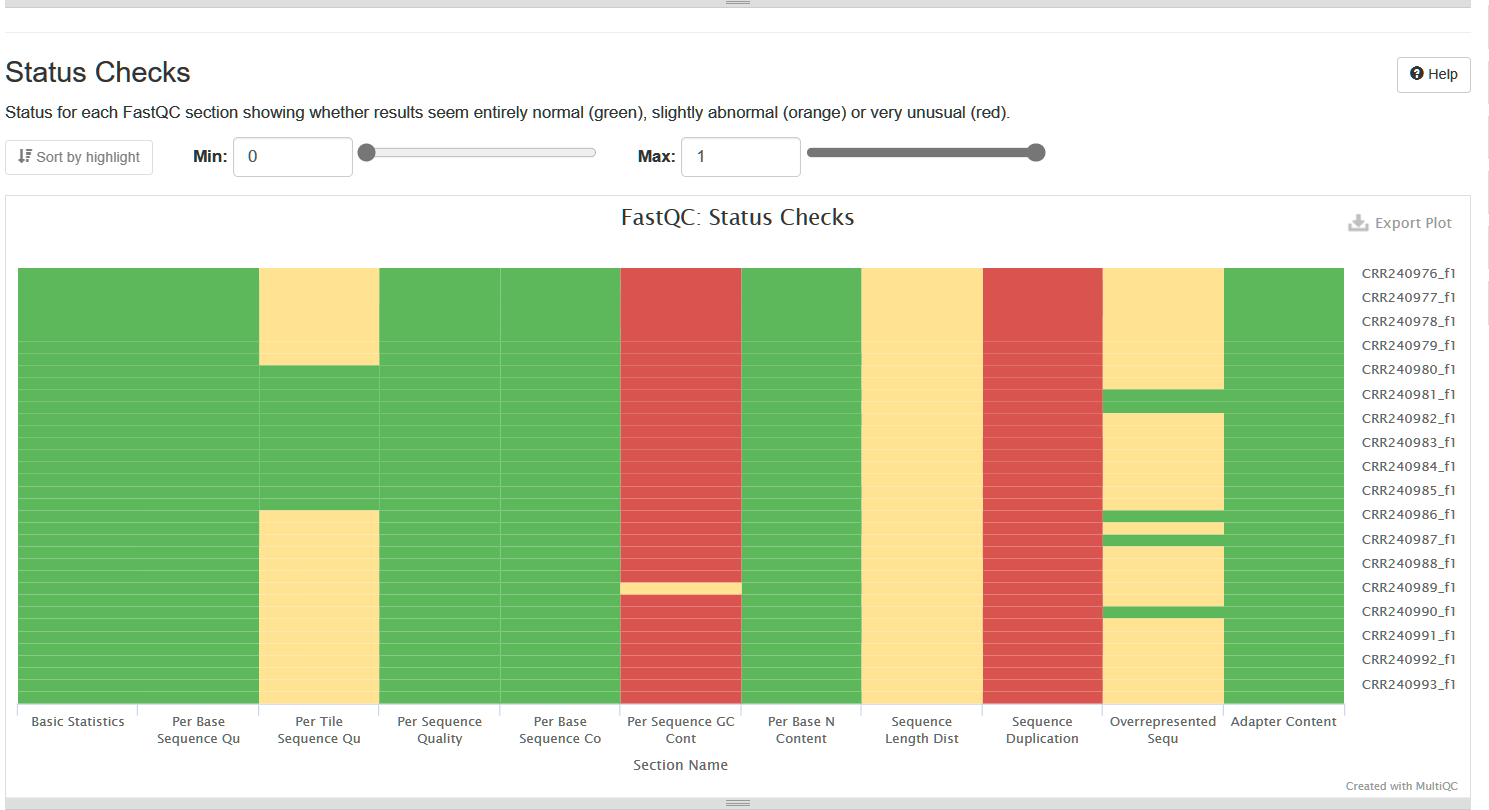
\includegraphics[width=\textwidth]{../../results/multiqc/Screenshots/0.1-MultiQC_FastQC_status_checks.png}
\end{figure}


TODO: Present the findings from the quality evaluation of the selected RNA-seq data.

\subsection{Mapping efficiency and coverage}
Report the results of the mapping process, including the mapping efficiency and coverage.

\subsection{Exploratory data analysis}
Discuss the dominating variance components, reproducibility, possible batch effects and confounding variables.

\subsection{Differentially expressed genes}
Discuss the identified differentially expressed genes and their potential biological significance.

\subsection{Functional enrichment analysis}
Present the results of the functional enrichment analysis, highlighting the enriched functional categories.